\documentclass[tikz]{standalone}
\begin{document}
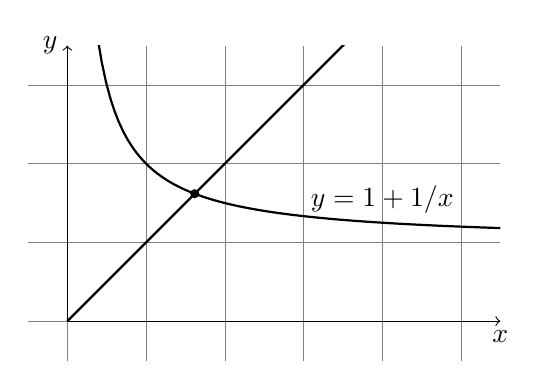
\begin{tikzpicture}
  \draw[help lines] (-0.5, -0.5) grid (5.5,3.5);
  \node [below] at (5.5,0) {$x$};
  \node [left] at (0,3.5) {$y$};
  %\node [below] at (1,1) {$y=x$};
  \node [above] at (4,1.25) {$y=1 + 1/x$};
  \draw [<->] (0, 3.5) -- (0, 0) -- (5.5,0);
  \begin{scope}
    \clip (-0.5,-0.5) rectangle (5.5,3.5);
    \draw[thick, domain=0.05:5.5, samples=100] plot (\x, {1 + 1/\x});
    \draw[thick, domain=0:5.5] plot (\x, {\x});
  \end{scope}
  \draw [fill] (1.618033988749895, 1.618033988749895) circle [radius=0.05];
\end{tikzpicture}
\end{document}
